This section will explain about the methodology, techologies and tools we used to develop the project. 
\subsection{Methodology}
%argumenter hvorfor for vi har valgt det.
%Tilpassinger, prsaker til tilpassinger.

This project has been developed using the Kanban-methodology which is a lean (and agile) development methodology. The nature of the project goes well with this methodology. With The goals of the project we had a high focus on making a working prototype. we focused on implementation. Something about incremental releasing. The implementation of user interface was not directly dependent on the application it self,  But in order to test it properly the rest of the application had to work. so we could work on these parts simultaneously. The ranking was implemented when the rest was more or less done. something about putting dependencies on the board we could ask the others to focus on that part. 
this way of working made it easy to make desisions along the way. we were all new to spring and had little knowleddge about the twitter api. so it was good for us to make a quick implementation to check if it worked.something about learning at the same time as implementing. Also a small project with few team members like our don't need to hold meetings on a regular basis like e.g in scrum. better to make the disisions when we needed.


being able to work on different part, puting the tasks on a board to see the dependencies.

This project has been developed using a Kanban. Kanban is a Lean software development methodology with five core principles:
Vizualize work flow 
Limit work in progress 
Manage flow
Make process policies explicite
Improve collaboration

At the start of the project we made a backlog of User Stories. We used an electronic kanban board from Kanbanpad.com to visualize the work flow. Through the development we split the stories into smaller development tasks and posted on the kanban board. This helped us limit the work in progress because we would finish a task before starting a new one. (See attachments for screenshots from the kanban board). The board also helped us kepp track of what the others were doing.

We used some tools and technologies in our development. 

\subsection{Tools} %snorre
During the project life cycle a number of tools have been used for the development process, implementation of code and deployment of the web application itself. A brief description of the tools used will be provided in this section.


\subsubsection{Workflow}
We adopted a lean and agile development workflow for our project using a Kanban-board, a version control system for rapid integration of new code/functionality and worked physically together as a team. We created a online Kanban-board at Kanbanpad.com. Kanbanpad is a free and online Kanban board with a simple interface and support for multiple platforms \cite{TheHybridGroup2012}.

\subsubsection{Implementation}
To implement the Java and Spring Framework based backend the SpringSource Tool Suite (Figure~\ref{fig:springsourcetoolsuite} was used. \textit{``SpringSource Tool Suite™ (STS) provides the best Eclipse-powered development environment for building Spring-powered enterprise applications.''} \cite{SpringSource}. SpringSource Tool Suite is built on the open-source IDE framework Eclipse, and provides functionality such as close integration with the Spring Framework, maven integration, automatic application deployment to web servers, debugging, code-completion and much more.

\begin{figure}[ht]
    \begin{minipage}[b]{1\linewidth}
        \centering
        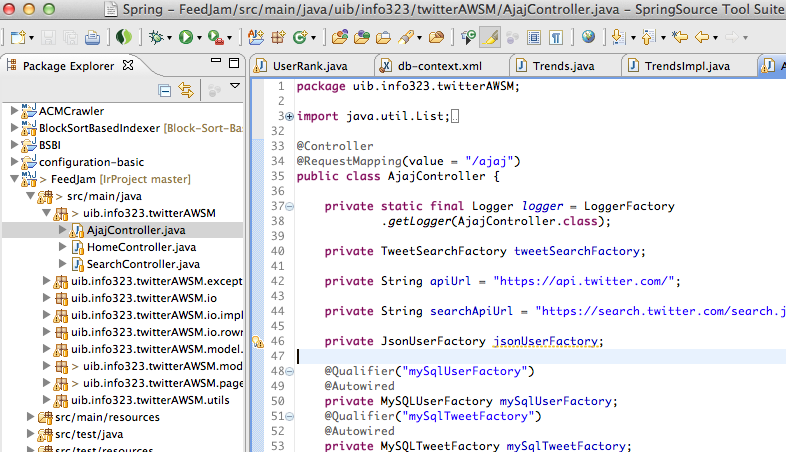
\includegraphics[width=1\textwidth]{figures/springsourcetoolsuite}
        \caption{The SpringSource Tool Suite IDE}
        \label{fig:springsourcetoolsuite}
    \end{minipage}
\end{figure}

The front-end code was implemented using mainly Notepad++ for coding and Google Chrome development tools for debugging and testing. \textit{``Notepad++ is a free (as in "free speech" and also as in "free beer") source code editor and Notepad replacement that supports several languages. Running in the MS Windows environment, its use is governed by GPL License.''} \cite{Ho2012}.

\subsubsection{Deployment}
The application is deployed on a server running the Linux-distro Ubuntu 12.04, a Tomcat web server, a LAMP-stack (Linux, Apache, MySQL, PHP) and Maven. Ubuntu 12.04 is the newest version of the operative system developed by Canonical and is suitable for use as a web server with desktop access. To serve the webpages of the FeedJam application we use Tomcat, an open-source webserver for Java-based web-applications. A MySQL server is used to drive the application's database of users and tweets. An Apache php server is used to provide the phpMyAdmin web interface to manage the MySQL server.

%Jeg vet ikke helt hva Torstein hadde tenkt å ha med her. Ble noe rart etter at jeg merget.

\subsection{Technology}
This section gives a short presentation of the techonologies we used in the project. 

\subsubsection{Javascript/jQuery} %torstein
This project relies heavily on client-side Twitter requests in order to provide each user with enough requests to make the application usable. Javascript is a scripting language, at the moment the only one, which is run client-side in browsers. While Javascript itself is quite straight forward, following the ECMAscript standard, there are several inconsistencies in its implementation in different browsers, leading to it demanding large amounts of experience in order to develop stable and functioning scripts. jQuery is a library written in Javascript which tries to account for these inconsistencies in addition to providing easier syntax and a large amount of prepared methods.

\subsubsection{Media Queries} %torstein
In order to customise the layout of websites for different screen resolutions one can employ the use of CSS media queries. While being a quite new innovation, media queries is supported by most browsers, including webkit and fennec based browsers, which includes most browsers used on smart phones and tablets. Media queries follow a quite simple syntax, and can be used within the standard css-document. For instance CSS written within "@media only screen and (min-width: 768px) and (max-width: 991px) \{" and "\}" would only be used in cases where the browser window has a width of between 768 and 991 pixels. 

Media queries are used in FeedJam in order to make the layout more available to smart phone and tablet users.

\subsubsection{AJAX}%torstein
AJAX, standing for Asynchronous Javascript and XML, is a technique where one can enable client-server interaction after a page has been rendered and send to the user's browser. In the context of our project we use the equivalent technique, AJAJ, which uses JSON instead of XML. On an abstract level one can explain AJAX as server requests which does not cause a page load, and whose response can be used either to insert new content dynamically or for some other purpose by the client.

\subsubsection{Media Queries} %torstein
In order to customise the layout of websites for different screen resolutions, and implement what we call a responsive design, one can employ the use of CSS media queries. While being a quite new innovation media queries is a part of the CSS3 standard \cite{W3C}. Media queries is supported by most browsers, including webkit and fennec based browsers, which includes most browsers used on smart phones and tablets. Media queries follow a quite simple syntax, and can be used within the standard css-document. For instance CSS written within "@media only screen and (min-width: 768px) and (max-width: 991px) \{" and "\}" would only be used in cases where the browser window has a width of between 768 and 991 pixels. Media queries are used in FeedJam in order to make the layout more available to smart phone and tablet users.

\subsubsection{JSON}
JSON (JavaScript Object Notation) is a data-interchange format \cite{Crockford2011}. JSON has several benefits when compared to other data-interchange formats such as XML. For instance, since it is based on Javascript object and array notation, it can be directly imported into Javascript. It is also lighter weight and arguably easier to write and read than the equivalent XML. In our project we receive data from the Twitter APIs in a JSON format.

\subsubsection{AJAX}%torstein
AJAX, standing for Asynchronous Javascript and XML, is a technique where one can enable client-server interaction after a page has been rendered and send to the user's browser \cite{Garrett2005}. In the context of our project we use the equivalent technique, AJAJ, which uses the JSON data format instead of XML. On an abstract level one can explain AJAX as server requests which does not cause a page load, and whose response can be used either to insert new content dynamically or for some other purpose by the client.

\subsubsection{jQuery Masonry}
Masonry is an open source jQuery plugin which enables better placement of elements within a grid.

\subsubsection{jQuery Revolver}
Revolver is an open source jQuery plugin which lets us generate a slider from a set of HTML elements.


\subsubsection{Spring} %lisa
To develop the project we used the Spring Framework. It is a Java based open source application framework. We chose this framework because it has many modules that easily takes care of the "plumbing" of the application and makes our work easier \citep{SpringSourcec}. Some of the group members has used it before, and all wanted to get to know it better because it one of the big enterprise frameworks. The application is set up using Spring MVC architecture which allows for easy communication between the web view and the controller (more on this in section \ref{} \nameref{}) \citep{SpringSourcee}. FeedJam uses Spring's REST module for client-side HTTP access to Twitter's API. We also make user of Spring's data access module for connection to the database.